\appendix

\chapter{An Example: TPC-H Query 6}
\label{appendix:full-query}

TPC-H query 6 is arguably the simplest of the 22 queries in the TPC-H benchmark. In this section, we will show how our query processor evaluates this query, and the various intermediate representations that are reached.

Figure \ref{fig:q6-sql} shows the SQL query that is inputted. This corresponds to box 1 in figure \ref{fig:translation-process}.

\begin{figure}[H]
    \centering
    \begin{tabular}{|c|}
    \hline
    \begin{lstlisting}[language=SQL]
SELECT
    sum("l_extendedprice" * "l_discount") as "revenue"
FROM
    "lineitem"
WHERE
    "l_shipdate" >= date '1994-01-01'
    AND "l_shipdate" < date '1994-01-01' + interval '1' year
    AND "l_discount" between 0.06 - 0.01 AND 0.06 + 0.01
    AND "l_quantity" < 24
    \end{lstlisting} \\
    \hline
    \end{tabular}
    \caption{TPC-H query 6 in SQL}
    \label{fig:q6-sql}
\end{figure}

\newpage

The first step is to generate a plan for this query, corresponding to box 2 in figure \ref{fig:translation-process}. This query is initially parsed into a very simple logical plan, shown in figure \ref{fig:q6-logical-plan}. This plan first does a table scan of the \texttt{lineitem} table, then a selection (\texttt{WHERE ...}), then a projection (of \texttt{l\_extendedprice * l\_discount}), and finally an aggregation (performing the \texttt{sum}).

Due to the simplicity of the initial plan, there is not a lot of optimisation we can do. As such, the plan is almost identical after rule-based logical optimisation, as you can see in figure \ref{fig:q6-optimal-plan}. However, we have recognised that we are capable evaluating the full query, and so every operator has been assigned a \texttt{Voodoo} calling convention.

\begin{figure}[H]
    \begin{subfigure}{0.49\textwidth}
        \centering
        \includegraphics[width=0.15\linewidth]{appendix/q6-logical-plan.png}
        \caption{Initial logical plan (before rule applications)}
        \label{fig:q6-logical-plan}
    \end{subfigure}
    \begin{subfigure}{0.49\textwidth}
        \centering
        \includegraphics[width=0.45\linewidth]{appendix/q6-plan.png}
        \caption{Optimised plan (after rule applications)}
        \label{fig:q6-optimal-plan}
    \end{subfigure}
    \caption{Calcite plan for TPC-H query 6}
    \label{fig:q6-plan}
\end{figure}

One thing that cannot be seen in the graphical representation of the plans in figure \ref{fig:q6-plan} are the row expressions, of which there are two. One represents the filter condition, shown in figure \ref{fig:q6-rex}, and the other represents the single projection, \texttt{l\_extendedprice * l\_discount}. During the logical optimisation stage, we apply rules to reduce constants in these row expressions, as shown.

\begin{figure}[H]
    \definecolor{light-purple}{RGB}{186, 161, 201}
    \definecolor{light-blue}{RGB}{187, 211, 249}
    \definecolor{light-red}{RGB}{255, 165, 165}
    \begin{subfigure}{0.98\textwidth}
    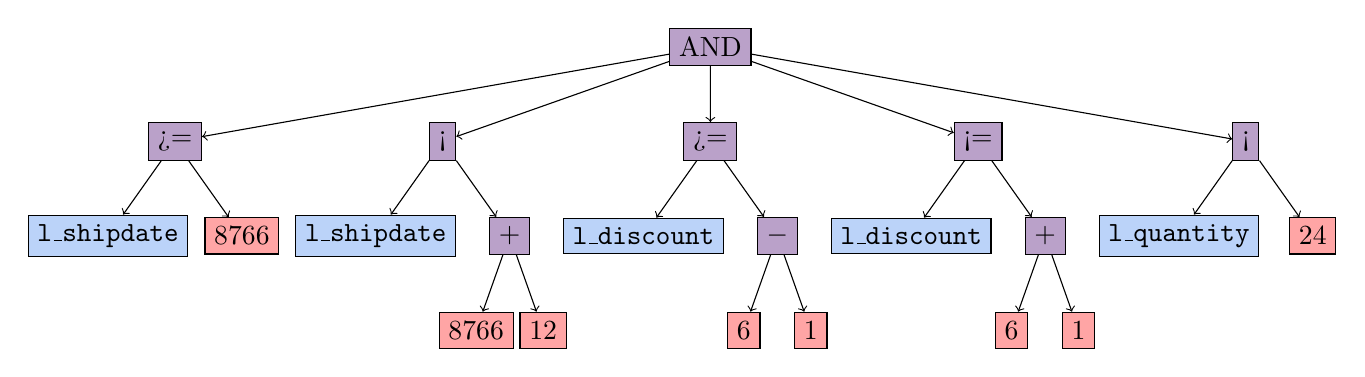
\begin{tikzpicture}[
        ->,
        level distance=1.2cm,
        every node/.style={shape=rectangle, draw, align=center},
        level 1/.style={sibling distance=3.4cm},
        level 2/.style={sibling distance=1.7cm}, 
        level 3/.style={sibling distance=0.85cm},
    ]
        \node[fill=light-purple] {AND}
            child { node[fill=light-purple] {>=}
                child { node[fill=light-blue] {\texttt{l\_shipdate}} }
                child { node[fill=light-red] {8766} }}
            child { node[fill=light-purple] {<}
                child { node[fill=light-blue] {\texttt{l\_shipdate}} }
                child { node[fill=light-purple] {$+$}
                    child { node[fill=light-red] {8766} }
                    child { node[fill=light-red] {12} }}}
            child { node[fill=light-purple] {>=}
                child { node[fill=light-blue] {\texttt{l\_discount}} }
                child { node[fill=light-purple] {$-$}
                    child { node[fill=light-red] {6} }
                    child { node[fill=light-red] {1} }}}
            child { node[fill=light-purple] {<=}
                child { node[fill=light-blue] {\texttt{l\_discount}} }
                child { node[fill=light-purple] {$+$}
                    child { node[fill=light-red] {6} }
                    child { node[fill=light-red] {1} }}}
            child { node[fill=light-purple] {<}
                child { node[fill=light-blue] {\texttt{l\_quantity}} }
                child { node[fill=light-red] {24} }};
    \end{tikzpicture}
    \centering
    \caption{Before rule applications}
    \end{subfigure}
    \\ [5ex]
    \begin{subfigure}{0.98\textwidth}
    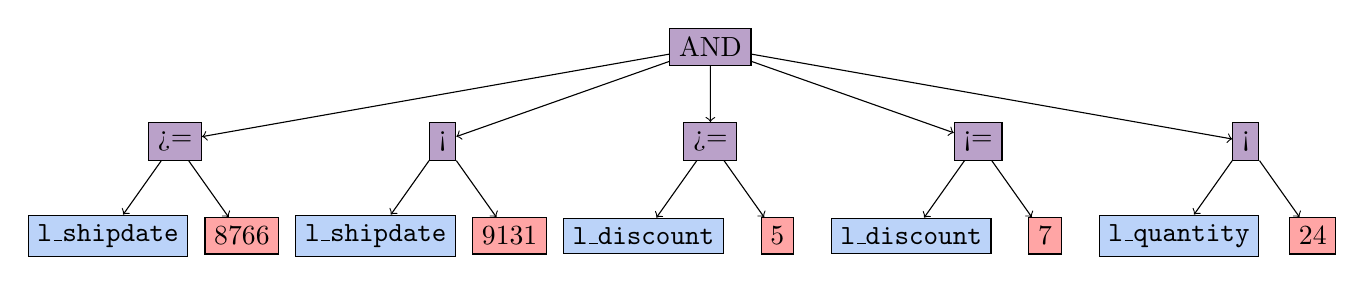
\begin{tikzpicture}[
        ->,
        level distance=1.2cm,
        every node/.style={shape=rectangle, draw, align=center},
        level 1/.style={sibling distance=3.4cm},
        level 2/.style={sibling distance=1.7cm}, 
        level 3/.style={sibling distance=0.85cm},
    ]
        \node[fill=light-purple] {AND}
            child { node[fill=light-purple] {>=}
                child { node[fill=light-blue] {\texttt{l\_shipdate}} }
                child { node[fill=light-red] {8766} }}
            child { node[fill=light-purple] {<}
                child { node[fill=light-blue] {\texttt{l\_shipdate}} }
                child { node[fill=light-red] {9131} }}
            child { node[fill=light-purple] {>=}
                child { node[fill=light-blue] {\texttt{l\_discount}} }
                child { node[fill=light-red] {5} }}
            child { node[fill=light-purple] {<=}
                child { node[fill=light-blue] {\texttt{l\_discount}} }
                child { node[fill=light-red] {7} }}
            child { node[fill=light-purple] {<}
                child { node[fill=light-blue] {\texttt{l\_quantity}} }
                child { node[fill=light-red] {24} }};
    \end{tikzpicture}
    \centering
    \caption{After rule applications}
    \end{subfigure}
    \centering
    \caption{Row expression for TPC-H query 6's filter condition}
    \label{fig:q6-rex}
\end{figure}

\newpage

The next stage of evaluation is to actually implement the plan in Voodoo algebra. This corresponds to box 3 in figure \ref{fig:translation-process}. By traversing the plan tree and the two row expression trees using visitor patterns, we produce the Voodoo algebra shown in figure. \ref{fig:q6-voodoo}.

\begin{figure}[H]
    \centering
    \includegraphics[width=\linewidth]{appendix/q6-voodoo.pdf}
    \caption{Voodoo vector expressions generated for TPC-H query 6}
    \label{fig:q6-voodoo}
\end{figure}

\newpage

Finally, we use these Voodoo API calls to build a Clang AST, as shown in figure \ref{fig:q6-ast}. This corresponds to box 4 in figure \ref{fig:translation-process}.

\begin{figure}[H]
    \centering
    \includegraphics[width=\linewidth]{appendix/q6-ast.png}
    \caption{Part of the AST generated for TPC-H query 6}
    \label{fig:q6-ast}
\end{figure}

From the AST, we generate the OpenCL code, shown in figure \ref{fig:q6-opencl}. This corresponds to box 5 in figure \ref{fig:translation-process}. The only change we have made to this code is to move arguments onto the following lines where necessary.

\begin{figure}[p]
    \centering
    \begin{tabular}{|c|}
    \hline
    \begin{lstlisting}[language=C]
__kernel void __runFragment0(__global int *persitent6, __global int *persitent10,
                             __global int *persitent13, __global int *persitent15,
                             __global long *persistent63) {
    struct {
        int fold;
        int value;
    } tmp38;
    int tmp39;
    struct {
        int fold;
        int value;
    } tmp59;
    int tmpAggregate60[32767] = {};
    int tmp61 = 0;
    for (int dominatingIteratorOffset = 0;
             dominatingIteratorOffset < 309;
             dominatingIteratorOffset += 1) {
        int tmp17 = 8766;
        int tmp18 = persitent6[dominatingIteratorOffset] > tmp17;
        int tmp19 = persitent6[dominatingIteratorOffset] == tmp17;
        int tmp20 = tmp18 || tmp19;
        int tmp21 = 9131;
        int tmp22 = tmp21 > persitent6[dominatingIteratorOffset];
        int tmp23 = 500;
        int tmp24 = persitent15[dominatingIteratorOffset] > tmp23;
        int tmp25 = persitent15[dominatingIteratorOffset] == tmp23;
        int tmp26 = tmp24 || tmp25;
        int tmp27 = 700;
        int tmp28 = tmp27 > persitent15[dominatingIteratorOffset];
        int tmp29 = persitent15[dominatingIteratorOffset] == tmp27;
        int tmp30 = tmp28 || tmp29;
        int tmp31 = 24;
        int tmp32 = tmp31 > persitent10[dominatingIteratorOffset];
        int tmp33 = tmp20 && tmp22;
        int tmp34 = tmp33 && tmp26;
        int tmp35 = tmp34 && tmp30;
        int tmp36 = tmp35 && tmp32;
        int tmp37 = dominatingIteratorOffset + 0;
        {
            tmp38.fold = tmp37;
            tmp38.value = tmp36;
        }
        {
            tmp39 = tmp38.value ? tmp38.fold : -1;
            if (tmp38.value) {
                int tmp52 = persitent13[tmp39];
                int tmp54 = persitent15[tmp39];
                int tmp56 = tmp52 * tmp54;
                int tmp57 = tmp56;
                int tmp58 = 1;
                {
                    tmp59.fold = tmp58;
                    tmp59.value = tmp57;
                }
                tmp61 = tmpAggregate60[tmp59.fold]
                      = tmpAggregate60[tmp59.fold] + tmp59.value;
            }
        }
    }
    int tmp62 = tmp61;
    persistent63[0] = tmp62;
}
    \end{lstlisting} \\
    \hline
    \end{tabular}
    \caption{OpenCL code generated for TPC-H query 6}
    \label{fig:q6-opencl}
\end{figure}

\chapter{The Apache Calcite Framework}
\label{appendix:calcite}

\subsubsection{Architecture of Apache Calcite}

\begin{figure}[H]
\includegraphics[width=0.4\textwidth]{appendix/calcite-architecture.png}
\centering
\caption{Architecture of Apache Calcite \cite{Begoli:2018:ACF:3183713.3190662}}
\label{fig:calcite-architecture}
\end{figure}

Calcite consists of most of the components needed to make a DBMS, with three significant omissions: algorithms to process data, storage of data, and a catalog for metadata. Figure \ref{fig:calcite-architecture} shows an overview of its architecture and interactions.

Firstly, Calcite provides a JDBC server (\emph{Avatica}), as well as a default implementation of its SPI. Alternatively, an application can use Avatica's JDBC driver directly (which is the approach we take with our web-interface).

Calcite then supports query evaluation in each of the following stages:
\begin{enumerate}
    \item \textbf{Parsing} the SQL query. Calcite provides an LL($k$) parser generated by JavaCC, and developers usually need not consider this step beyond setting some basic configuration options.
    \item \textbf{Validating} the SQL query. Calcite validates queries against any known metadata. Developers need to provide an interface that allows Calcite to get this metadata for a table (an \emph{adapter}).
    \item \textbf{Optimising} the logical plan, and converting it to physical expressions. Calcite can do this with some help. It provides two algorithms for rule-based logical query optimisation, as well as around one-hundred rules. However, developers will likely need to add further rules, including rules to rewrite a logical plan into physical expressions for their application.
    \item \textbf{Executing} the physical plan, by converting it into application-specific executions. Calcite can handle this in simple cases, say where the application actually supports SQL input (i.e. Calcite is just being used as an optimiser). In other cases, such as ours, this step requires a lot of application-specific code to be written.
\end{enumerate}

\subsubsection{Relational algebra}
\label{rel}

Calcite uses relational algebra \cite{Codd:1970:RMD:362384.362685} to express queries. Specifically, it builds a tree of \texttt{RelNode}s, each of which represent a relational operator. Each \texttt{RelNode} could represent, for example, a \texttt{TableScan}, \texttt{Project}, \texttt{Filter}, \texttt{Aggregate}, \texttt{Join}, \texttt{Union}, \texttt{Intersect} or \texttt{Sort}.

Projection and sort fields, as well as filter and join conditions, are expressed by trees of \texttt{RexNode}s. A \texttt{RexNode} represents a row-level expression, and its implementations include \texttt{RexCall} (an operation such as "add" or "is equal to"), \texttt{RexInputRef} (a reference to an input column) and \texttt{RexLiteral} (a literal value), as well as many others (which we do not consider).

Relational expressions are associated with \emph{traits} (\texttt{RelTrait}s), which describe their physical properties, such as ordering, grouping, or partitioning. The most important trait, however, is the \emph{calling convention} (\texttt{Convention}), which specifies the data processing system where the expression will be executed. The \texttt{Logical} calling convention is used when no implementation has been selected.

\subsubsection{Query processing and optimisation}

Calcite includes \emph{planner rules} (\texttt{RelOptRule}s) to transform expression trees. Each rule defines a condition on the original tree, and a conversion, that rewrites part of the tree. Calcite provides common rules, such as the \texttt{FilterIntoJoinRule}, which pushes a filter into a join where possible, to reduce the work in the join. Developers also must provide their own rules to transform the tree from a logical to an optimised physical plan.

Calcite also provides two planner engines (\texttt{RelOptPlanner}s) to apply these rules: one requires a cost-model and uses a dynamic programming algorithm, similar to Volcano's \cite{Graefe:1994:VEP:627290.627558} (\texttt{VolcanoPlanner}), whilst the other exhaustively applies rules until it reaches a fixpoint (\texttt{HepPlanner}).

\subsubsection{Adapters}

\begin{figure}[H]
\includegraphics[width=0.42\textwidth]{appendix/calcite-adapter.png}
\centering
\caption{A minimal adapter for Apache Calcite \cite{Begoli:2018:ACF:3183713.3190662}}
\label{fig:calcite-adapter}
\end{figure}

As Calcite does not include a storage layer, it requires developers to build an \emph{adapter}. Figure \ref{fig:calcite-adapter} shows the design of a minimal adapter:
\begin{itemize}
    \item The \texttt{Model} is a JSON-formatted description of the physical properties of the data source being accessed.
    \item The \texttt{Schema} is a definition of the data found in the model, and is generated by a \texttt{SchemaFactory} for the adapter. Usually this will use a \texttt{TableFactory}, which generates a \texttt{Table} defining the names and types of the columns in each table, as well as any statistics available, such as cardinalities, distributions, and which columns are keys.
\end{itemize}

An adapter also usually provides a set of rules to be added to the planner. Specifically, rules to rewrite logical operators to physical operators of the adapter's convention.

The minimal rule set includes a translation for table-scans, which implement the access paths for tables in the adapter. Once Calcite can read the data, it can implement all other operators using the \texttt{Enumerable} calling convention, which uses a conventional iterator implementation written in Java.

Rules are also used to convert all other operators, to avoid plans relying too heavily on costly \texttt{Enumerable} operators. Each of these rules, in our case, defines an implementation instead using the \texttt{Voodoo} convention.

\chapter{Relational Operator Implementations}
\label{appendix:rel}

\begin{enumerate}
    \item \textbf{Table scans}
    
    \texttt{TableScan} is a relatively simple operator that can access a \texttt{VoodooTable}, and \texttt{Import}, \texttt{Persist} and \texttt{Load} its column vectors into the back-end's memory.

    \item \textbf{Projections}
    
    \texttt{Project} is a similarly simple operator. Each projected field is defined as a row expression and is implemented as described in subsection \ref{sub:rex}. The final result is then made available for the parent node to access.

    \item \textbf{Filters}

    \begin{figure}[H]
        \centering
        \includegraphics[width=0.75\linewidth]{appendix/filter.pdf}
        \caption{Implementing $\sigma_{\text{COL} < 2 \lor \text{COL} > 3}\text{COL}'$ in Voodoo vector algebra}
        \label{fig:filter}
    \end{figure}
    
    \texttt{Filter} represents a selection in relational algebra. To implement a filter, we first implement its condition, which is a row expression. This should return a vector of zeroes and ones, where the ones correspond to rows which should be selected. Figure \ref{fig:filter} shows an example of this, where we have reached the vector labelled "$*$". We \texttt{Zip} this condition vector with the row indices of the table. We then use a \texttt{FoldSelect}, which selects the indices corresponding to non-zero values in the condition vector. These indices are then used to \texttt{Gather} the selected rows from each column of the table.
    
    The final result has non-selected rows as empty-slots, shown as "$/$" in the figure. In reality, these are "junk" values, and are difficult to distinguish in some cases. As such, in addition to the resulting vectors, we always keep a reference to the condition vector ($*$), which allows us to determine exactly which rows were selected.
    
    \item \textbf{Aggregates}
    
    \texttt{Aggregate} represents a grouped aggregation in relational algebra. Currently, we support the \texttt{SUM}, \texttt{COUNT}, \texttt{MIN}, \texttt{MAX} and \texttt{AVG} aggregate functions applied without grouping (i.e. for the entire column). We will describe a \texttt{SUM} here, but it is clear to see that the other operators would be implemented similarly. To implement this operator, we must first implement the specified row expression, which should return a vector containing the values from the specified column with the expression applied to each value. We then \texttt{zip} this vector with a run-vector which contains all ones. A \texttt{foldSum} is then applied to this, which generates a new vector containing the sum of all the values in each run in the run vector (in this case, we have a single run, so all values are summed). Finally, we \texttt{project} this final vector onto the specified alias specified. Figure \ref{fig:aggregate} shows an example of this.
    
    \begin{figure}[H]
        \centering
        \includegraphics[width=0.5\linewidth]{appendix/aggregate.pdf}
        \caption{Implementing $\Gamma_{(\text{COL} \times 2, (\{\}, \texttt{SUM}))}$ in Voodoo vector algebra}
        \label{fig:aggregate}
    \end{figure}
    
    Although currently not fully implemented, supporting grouping would involve a \texttt{partition} of the group key\footnote{For multiple group keys, we need use \texttt{BitShift} and \texttt{BitwiseOr} operations to combine the group key vectors together as a single vector, and use this result as the group key.} using a vector of indices. We will call the result of this operation \texttt{A}. Then, we \texttt{scatter} the vector \texttt{A} with respect to the group key - let this result be the vector \texttt{B}. We also \texttt{scatter} the vector \texttt{A} with respect to the vector of values which we want to apply the aggregate function to - let this result be the vector \texttt{C}. After, we \texttt{zip} the vectors \texttt{B} and \texttt{C} and apply \texttt{foldSum} to this (now using \texttt{B} as the run-vector, instead of just a constant vector of ones). An example of this is shown in figure \ref{fig:group-by}.
    
    Since the empty slots in this case may be difficult to determine, we could \texttt{scatter} a vector of ones into a vector zeroes using the group key as the pivots, in order to produce a column allowing us to determine exactly which rows form the result.
    
    \begin{figure}[H]
        \centering
        \includegraphics[width=0.75\linewidth]{appendix/group-by.pdf}
        \caption{Implementing $\Gamma_{(\text{Column}, (\text{Group key}, \texttt{SUM}))}$ in Voodoo vector algebra}
        \label{fig:group-by}
    \end{figure}
    
    \item \textbf{Joins}
    
    \texttt{Join} is a rather difficult operator to implement. We have currently implemented the most simple case, which is just a cross product (i.e. a join with no condition). We apply \texttt{Cross} to a vector from the first relation with a vector from the second relation. After, we use the result in a \texttt{Gather}, with the columns being projected. If the join has a condition, we can then apply the filter (see above) with the join condition.
    
    We also have an implementation which may be used when there is a foreign key relationship, referring to a primary key that is known to be dense. In this case, all that is required is to \texttt{Subtract} the offset of the dense key column, and apply a \texttt{Gather}.
    
    One thing to note is that if a join is performed on columns that have been filtered, it can be difficult to tell which rows should be returned in the final result. One solution is to never push filters inside joins, which would completely avoid this issue. Another is to use the condition columns, which \texttt{Filter}s keep a reference to, and apply \texttt{Gather}s and logical vector operations to work out which columns in the join result should be filtered.
    
\end{enumerate}

\chapter{Voodoo API Implementation}
\label{appendix:api}

\begin{enumerate}

\item \texttt{Import(vector v1)}

This loads a vector holding input data (in the form of a pointer to a buffer) into the \texttt{VectorProcessor}. This vector is now referred to as a persistent or input vector.

\item \texttt{Load(vector v1)}

This loads a previously created persistent vector and allows other calls to access the data held within it. It registers the persistent vector as being present in the parameters to the final fragment. 

This generates a \texttt{Clang::ParmVarDecl} declaring the name and type of the vector in the fragments function parameters.

\item \texttt{Project(vector v1, KeyPath k1)}

This projects a loaded vector and allows other calls to access the data held within it. It leads to the generation of the dominating iterator for loop that is used to cycle through the values of the projected vector. If the vector v1 contains multiple members, then KeyPath k1 is used to access the specific member, otherwise it is ignored.

This generates a \texttt{Clang::DeclStmt} declaring and initialising the vector. E.g.

{\centering\texttt{tmp1 = v1[dominatingIterator].k1}\par}

\item \texttt{Gather(vector v1, positions)}

\texttt{Gather} is a more complicated version of project. Instead of cycling through all the values of a vector it takes in another vector (positions) which it uses as the indices of the vector to access. 

This generates a \texttt{Clang::DeclStmt} declaring and initialising the vector. E.g. 

{\centering\texttt{tmp1 = v1[positions[dominatingIterator]]}\par}

\item \texttt{LogicalAnd(vector v1, v2)}, \texttt{LogicalOr(vector v1, v2)}, \texttt{BitwiseAnd(vector v1, v2)}, \texttt{BitiwseOr(vector v1, v2)}, \texttt{Equals(vector v1, v2)}, \texttt{Add(vector v1, v2)}, \texttt{Subtract(vector v1, v2)}, \texttt{Greater(vector v1, v2)}, \texttt{Modulo(vector v1, v2)}, \texttt{Divide(vector v1, v2)}

All of these Voodoo API calls take two vectors of identical size and perform a single operation on them, outputing a single vector of the same size. 

This generates a \texttt{Clang::DeclStmt} declaring and initialising the vector. E.g.

{\centering\texttt{tmp1 = v1 (+ / - / * / == / ...) v2}\par}

\item \texttt{BitShift(vector v1, v2)}

This take two vectors of identical size and shifts the first by the second amount. If the amount is positive it is a right shift otherwise it is a left shift. This outputs a single vector of the same size.

\item \texttt{Range(int/long/float min, count, step)}

\texttt{Range} generates a vector of size count, representing a range of numbers, starting at min and increasing by count between each number. Count can also be input as a vector, and range will generate a vector of identical size to count. 

This generates a \texttt{Clang::DeclStmt} declaring and initialising the vector. E.g.

{\centering\texttt{tmp1 = min + step * dominatingIterator}\par}

\item \texttt{Zip(vector v1, v2, KeyPath k1, k2)}

\texttt{Zip} takes two vectors of identical size and zips them together into one vector. The output vector will contain vector \texttt{v1} in KeyPath \texttt{k1} and vector \texttt{v2} in KeyPath \texttt{k2}. This is necessary for the fold operations, which require a zipped vector, and utilise KeyPath to access them.

This generates a \texttt{Clang::DeclStmt} declaring and initialising the vector. E.g.

{\centering\texttt{tmp1 = \{{k1: v1, k2: v2\}}}\par}

\item \texttt{FoldSelect(vector v1, KeyPath fold, val)}

\texttt{foldSelect} takes a vector and branches via an if statement based on the val of the vector. Returning \texttt{v1.fold} if \texttt{v1.val} is non-zero, otherwise returning -1. Any further statements using the output of the \texttt{foldSelect} will be placed inside the if statement.

This generates multiple \texttt{Clang::Stmts}, generating the output of the \texttt{foldSelect} and the branch:

{\centering\texttt{tmp4 = tmp3.value ? tmp3.fold : -1; if (tmp3.value) \{{...\}}}\par}

\item \texttt{FoldSum(vector v1, KeyPath fold, val)}, \texttt{FoldMax(vector v1, KeyPath fold, val)}, \texttt{FoldMin(vector v1, KeyPath fold, val)}

\texttt{foldSum}/\texttt{Max}/\texttt{Min} takes a vector and computes the sum / max / min of the val based on the fold attribute. This generates a \texttt{Clang::Stmt} assigning:

{\centering\texttt{tmp7 = tmpAggregate6[tmp5.fold] = tmpAggregate6[tmp5.fold] + tmp5.value;}\par}

This will "reduce" a vector to a single value. 

\item \texttt{Cross(vector v1, v2)}

\texttt{Cross} generates a nested for loop, looping through the values of \text{v2}. This allows data from one table to be crossed with another table. During the block generation process this manifests as a block contained within another block.

This generates a \texttt{Clang::Stmt} declaring the for loop:

{\centering\texttt{for(int dominatingIteratorOffset2 = 0; i < v2.size; i++) \{{...\}}}\par}

and allows future calls to access the new iterator to loop through the values of v2.

\item \texttt{ReturnVector(vector v1)}

\texttt{ReturnVector} projects a vector into a new output vector with a buffer to hold the final output values. This adds the output vector to the parameter list so the buffer location can specified at runtime by the \texttt{VectorProcessor}. This invokes the fragment generation code and generates the final code to be run in addition to the output size and type, storing it in the vector. This generates a \texttt{Clang::Stmt} assigning the vector. E.g.

{\centering\texttt{persistent1[0] = v1} or \texttt{persistent1[dominatingIterator] = v1}\par}

and a \texttt{Clang::ParmVarDecl} declaring the name and type of the vector in the fragments function parameters. This returns the vector, ready to be resolved (ran) and for the values to be read.

\item \texttt{ReturnMultiVector(list of vectors vs)}

This generates multiple return statements, adding each return statement to the fragment as well as each output buffer and then generating the code for this fragment. The final code is stored in the first vector. When the list of vectors is resolved, only the first vector is run, but all output buffers from the list are registered to OpenCL and so all output vectors are populated. 

This returns a list of vectors, ready to be resolved and for the values of each vector to be read.

\item \texttt{Resolve(vector or list of vectors)}

This runs the given vectors, passing input and output buffers to the \texttt{VectorProcessor} and then returning the vectors containing the results back to the user.

This call will only work on vectors produced from previous calls to \texttt{ReturnVector} or \texttt{ReturnMultiVector}.
 
Once the relevant Clang statements have been created, they are added to the \texttt{AstVector}. The \texttt{AstVector} also stores the \texttt{AstVector}s that this function requires.

\item \texttt{Partition(vector v1, vector v2)}

Partition takes an input vector v1 and a list of pivots v2. It loops through the input vector, and for each value, increment the size of the histogram bin the input belongs in. The semantics is defined such that the input value goes in the bucket that has a pivot greater the input value. Then iterate through the histogram array and work out the starting positions using a prefix sum and set the sizes back to zero. Each of these steps can be done in parallel. \cite{Maleki:2016:HTM:2980983.2908089}
Using the histogram start and size values, it returns the pivot that is assigned to the input vector. This essentially outputs the positions of the input values if they were ordered(\texttt{vector v3}). There are cases where this can be simplified.

An example of just the working out the pivot for the input value is presented below. 

{\centering\texttt{v3.val = v3Histogram[v1.val \& 31].start + v3Histogram[v1.val \& 31].size++;}\par}


\item \texttt{Scatter(vector v1, vector v2, vector v3)}
Scatter takes an input vector v1, an output vector v2 and a list of pivots v3. It loops through the values in input, placing them in the corresponding pivot position in the output vector. On conflict, values are overwritten in the output vector. Scatter breaks the current block, as a full iteration through the input vector is required to correctly generate the output vector. This generates a \texttt{Clang::Stmt} assigning the vector. E.g.

{\centering\texttt{v1[v2] = v3}\par}

\end{enumerate}

\chapter{Generating Blocks for \texttt{FoldSelect}}

Dealing with the \texttt{foldSelect} block is slightly different as it creates an if statement instead of a typical for loop statement. Any calls following the \texttt{foldSelect} will be inserted inside the if statement. 

If a reducer is called in the \texttt{foldSelect} scope, this needs to close the if statement (if it is a nested \texttt{foldSelect}, then close all the if statements) and then close the for loop the if statement belongs in. Figure \ref{fig:fragmentConstructionfoldSelect} shows a step by step process of how the blocks are created for the query in figure \ref{fig:ASTfoldSelect}. All folds require a zip and a range call before they can be used. These calls have been omitted for brevity.

\begin{figure}[h]
  \centering
  \includegraphics[width=\textwidth]{appendix/foldSelectQuery.pdf}
  \caption{A foldSelect Query which sums together all the quantities which have a non-zero order key}
  \label{fig:ASTfoldSelect}
\end{figure}%

\begin{figure}[h]
\centering
\includegraphics[width=1\linewidth]{appendix/FragmentConstructionFoldSelect.pdf}
\caption{Block Construction for a foldSelect Query. \ref{fig:ASTfoldSelect}}
\label{fig:fragmentConstructionfoldSelect}
\end{figure}

\begin{figure}
\begin{lstlisting}[frame=single, language=C]
__kernel void __runFragment0(
    __global int *persitent1, // L_QUANTITY column vector
    __global int *persitent3, // L_ORDERKEY column vector
    __global long *persistent10 // Result vector
) {
    struct {
        int fold;
        int value;
    } tmp5;
    int tmp6;
    int tmpAggregate7[32767] = {};
    int tmp8 = 0;
    for (int dominatingIteratorOffset = 0; 
         dominatingIteratorOffset < 3; 
         dominatingIteratorOffset += 1) {
        int tmp2 = persitent1[dominatingIteratorOffset];
        int tmp4 = persitent3[dominatingIteratorOffset];
        {
            tmp5.fold = tmp2;
            tmp5.value = tmp4;
        }
        {
            tmp6 = tmp5.value ? tmp5.fold : -1;
            if (tmp5.value) {
                tmp8 = tmpAggregate7[tmp6] = tmpAggregate7[tmp6] + tmp6;
            }
        }
    }
    int tmp9 = tmp8;
    persistent10[0] = tmp9;
}
\end{lstlisting}
    \caption{OpenCL code for \ref{fig:ASTfoldSelect}}
    \label{fig:openclCodeFoldSelect}
\end{figure}

\chapter{A Dynamic Programming Algorithm for Generating Blocks}
\label{appendix:dpalgo}
The current implementation of the block creation is a recursive algorithm. The problem of grouping statements together by the scope they belong to has an optimal substructure and there exists overlapping sub problems. An attempt has been made to convert the recursive solution into a dynamic programming solution.

Let us take the query represented in Figure \ref{fig:DPSimpleQuery}, specifically the \texttt{Zip} node. \texttt{Zip} operates on two vectors which in this case point to the same \texttt{Project} statement. The current implementation would recurse up the first vector and create a block and add the \texttt{Load} and \texttt{Project} statements. Once it has finished creating the block, it would recurse up the second vector that \texttt{Zip} depends upon, create a new block and add the same \texttt{Load} and \texttt{Project} call to that block. The algorithm would try and merge the blocks together and then proceed to add the \texttt{Zip} statement to the new merged block. This process is shown in figure \ref{fig:DPSimpleQueryFrag}.

An easy way to fix recursing over overlapping sub problems, is to use memoisation: have a map from the statement to the block it belongs in. If the statement already exists in a block, then return that block, instead of recreating it and merging it. This naive dynamic programming algorithm, has been implemented.

\begin{figure}
    \centering
    \begin{subfigure}{0.5\linewidth}
        \centering
        \includegraphics[width=0.5\linewidth]{appendix/DPExplain.pdf}
        \caption{An example query to show that there exists overlapping sub problems and has an optimal substructure}
        \label{fig:DPSimpleQuery}
    \end{subfigure}
    \begin{subfigure}{\linewidth}
        \centering
        \includegraphics[width=0.5\linewidth]{appendix/DPExplainFrag.pdf}
        \caption{The process of creating blocks and merging blocks using the recursive solution before the zip statement can be added}
        \label{fig:DPSimpleQueryFrag}
    \end{subfigure}
    \caption{Caption}
    \label{fig:my_label}
\end{figure}

The case which our implemented naive dynamic programming algorithm does not handle, is the case presented in figure \ref{fig:dpedgeCase}. The figure shows what the final block creation looks like with the recursive algorithm. 


Using the naive dynamic programming algorithm, the algorithm would recurse up to the \texttt{Zip} statement. Then recurse up the first \texttt{requiredVector} and create the block (with block number 1) for the \texttt{Load}, \texttt{Project} and \texttt{FoldSum} statements. Once that block is created, the algorithm would recurse up the second \texttt{requiredVector} which in this case is a \texttt{Project} statement. As the \texttt{Project}'s \texttt{requiredVector} is a \texttt{Load} statement which already exists in block 1, it will return block 1 and add the \texttt{Project} statement to it. This is wrong! Instead of returning block 1, it should create a new block. This is because block 1 is reduced and the Zip statement depends on the result of the foldSum and therefore the zip statement and the block created from it's 2\textsuperscript{nd} \texttt{requiredVector} cannot belong with block 1 as it violates the 3rd condition to merge blocks. Figure \ref{fig:dpedgeCaseNaive} shows what the final block creation looks like with the naive dynamic programming algorithm. 

The block that will be created by the 2\textsuperscript{nd} \texttt{requiredVector} of the \texttt{Zip} statement is not aware about which blocks it can use to insert statements with or merge with. 

A possible solution is to pass a set of blocks that the 2\textsuperscript{nd} \texttt{requiredVector} cannot use and if a statement exists in the map, retrieve the block and check to see if that block is in the list banned blocks. If it is then create a new block instead of using the retrieved block.

Another possible solution, is to guarantee that unique load calls will be made for each set of statements that belong in the same scope. If this can be guaranteed, then the naive dynamic programming solution will work.

\begin{figure}
    \centering
    \begin{subfigure}{\textwidth}
        \includegraphics[width=\textwidth]{appendix/DPEdgeCase.pdf}
        \caption{An example query used to explain the edge case that is not handled by the naive dynamic programming algorithm. It also shows what the final stage of the blocks should look like using the recursive algorithm}
        \label{fig:dpedgeCase}
    \end{subfigure}
    \begin{subfigure}{0.6\textwidth}
        \centering
        \includegraphics[width=0.5\linewidth]{appendix/DPNaive.pdf}
        \caption{Blocks created when the naive dynamic programming algorithm is used}
        \label{fig:dpedgeCaseNaive}
    \end{subfigure}
\end{figure}

\chapter{Metrics}
\label{appendix:metrics}

\section{Test Coverage}

\begin{figure}[H]
    \centering
    \includegraphics[width=0.7\linewidth]{evaluation/frontend-coverage.png}
    \caption{Font-end test coverage}
    \label{fig:fontend-cov}
\end{figure}

\begin{figure}[H]
    \centering
    \includegraphics[width=0.75\linewidth]{evaluation/backend-coverage.png}
    \caption{Back-end test coverage.}
    \label{fig:backend-cov}
\end{figure}

\section{\texttt{Metrix++} results}

\begin{table}[H]
    \centering
    \begin{tabular}{@{}lllll@{}}
        \toprule
        \textbf{Metric}       & \textbf{Max} & \textbf{Avg} & \textbf{Total} \\ \midrule
        Cyclomatic Complexity & 71           & 1.29         & 1760           \\
        Maximum Indentation   & 11           & 1.41         & 1925           \\
        Magic Numbers         & 179          & 4.28         & 1341           \\ \bottomrule
    \end{tabular}
    \caption{\label{table:original-metrics}Original code results}
\end{table}

\begin{table}[H]
    \centering
    \begin{tabular}{@{}lllll@{}}
        \toprule
        \textbf{Metric}       & \textbf{Max} & \textbf{Avg} & \textbf{Total} \\ \midrule
        Cyclomatic Complexity & 71           & 1.86         & 820           \\
        Maximum Indentation   & 5            & 1.42         & 624            \\
        Magic Numbers         & 15           & 3.02         & 348           \\ \bottomrule
    \end{tabular}
    \caption{\label{table:opencl-metrics}\texttt{OpenCL} implementation results}
\end{table}

\begin{table}[H]
    \centering
    \begin{tabular}{@{}lllll@{}}
        \toprule
        \textbf{Metric}       & \textbf{Max} & \textbf{Avg} & \textbf{Total} \\ \midrule
        Cyclomatic Complexity & 24           & 1.05         & 128            \\
        Maximum Indentation   & 6            & 1.66         & 202           \\
        Magic Numbers         & 25           & 3.03         & 100           \\ \bottomrule
    \end{tabular}
    \caption{\label{table:clangast-metrics}\texttt{ClangAst} implementation results}
\end{table}

\paragraph{Disclaimer} These values should be taken with a pinch of salt. There are significant differences between the implemented algorithms, and different style choices were made.

Furthermore, the metric \emph{Magic Numbers} includes \textbf{0}s and \textbf{1}s and we do not know how \texttt{Metrix++} implements cyclomatic complexity.

\chapter{Dependencies}

\begin{table}[h]
    \centering
    \begin{tabular}{l l l}
        \hline
        \textbf{Repository} & \textbf{Dependency} & \textbf{License} \\
        \hline
        \texttt{calcite}    & Apache Calcite & Apache License 2.0 \\
        \texttt{calcite}    & Guava          & Apache License 2.0 \\
        \texttt{calcite}    & JUnit          & Eclipse Public License 1.0 \\
        \texttt{calcite}    & sqlline        & 3-Clause BSD License \\ 
        \hline
        \texttt{voodoo}     & Clang          & University of Illinois/NCSAOpen Source License \\
        \texttt{voodoo}     & OpenCL         & Khronos Specific License \\
        \texttt{voodoo}     & Boost          & Boost Software License \\
        \texttt{voodoo}     & Googletest     & 3-Clause BSD License \\
        \hline
        \texttt{voodoo-vis} & Axios          & MIT License \\
        \texttt{voodoo-vis} & Buefy          & MIT License \\
        \texttt{voodoo-vis} & Codemirror     & MIT License \\
        \texttt{voodoo-vis} & VisJS          & May be distributed under MIT or Apache 2.0 \\
        \texttt{voodoo-vis} & VueJS          & MIT License \\
        \hline
    \end{tabular}
    \caption{\label{table:dependencies}Licenses for each library used}
\end{table}

All software and packages detailed above are under licenses which would allow commercial use.

If this project was to be open-sourced, any copies of packages must include the original copyright texts and licenses (should we choose to distribute them along with our own source).
